\subsection{Strategy Pattern}

\subsubsection*{Problembeschreibung}

Es kann vorkommen, dass mehrere Varianten eines Algorithmus benötigt werden, welche ein einheitlichen Iinterface bereitstellen. Je nach Kontext wird ein anderer Algorithmus benötigt. Die Algorithmen sollen dynamisch austauschbar sein, um deren flexiblen Einsatz zu ermöglichen und eine lose Kopplung zu gewährleisten. Eine Implementierung der Algorithmen-Varianten innerhalb der ausführenden Klasse, würde deren Komplexität deutlich erhöhen. Außerdem soll die Möglichkeit bestehen, in Zukunft weitere Algorithmen hinzuzufügen. Das Strategy-Pattern kann die Übersichtlichkeit verbessern, wenn viele ähnliche Klassen existieren, die sich lediglich in ihrem verhalten unterscheiden. Weiterhin werden Implementierungsdetails und Algorithmus-spezifische Daten vom Kontext abgekapselt.

\subsubsection*{Lösung}

Der Context besitzt eine Referenz auf eine Strategie. Die konkrete Strategie wurde dem Context zuvor durch den Client zugewiesen. Die konkrete Strategie realisiert das Strategy-Interface, sodass Context und konkrete Strategie lediglich lose gekoppelt sind. Jede Strategie stellt die Methode `execute` bereit, um den gekapselten Algorithmus auszuführen. 

\begin{figure}[!hb]
	\centering
	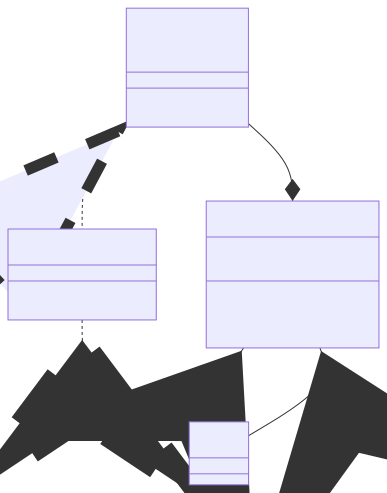
\includegraphics[width=0.75\linewidth]{images/patterns/strategy-class.png}
	\caption{Klassendiagramm Strategy Pattern}
	\label{fig:strategy-class}
\end{figure}

Der Context wird initialisiert, indem ihm vom Client eine konkrete Strategie zugewiesen wird (3), welche zuvor vom Client erstellt wurde (1). Der Client kann von nun an den Context dazu veranlassen, eine Aktion durchzuführen, welche die Verwendung des in der hinterlegten Strategie hinterlegten Algorithmus nach sich zieht (5). Der Context kann den Algorithmus ausführen (6), ohne Wissen über die konkrete Strategie zu benötigen. 

\begin{figure}[!hb]
	\centering
	\includegraphics[width=0.75\linewidth]{images/patterns/strategy-seq.png}
	\caption{Sequenzdiagramm Strategy Pattern}
	\label{fig:strategy-seq}
\end{figure}

\subsubsection*{Konsequenzen}
Das Strategy-Pattern ermöglicht es, durch die Verwendung von Vererbung eine Hierarchie von Algorithmen aufzubauen. Das kann hilfreich sein, wenn mehrere Algorithmen sich Teile ihrer Implementierung teilen. Das Pattern extrahiert die Algorithmen-Implementierung aus dessen Kontext und verhindert damit die sonst notwendige Bildung von Subklassen des Kontextes. Die Auswahl des auszuführenden Algorithmus wird über Aggreation gesteuert. Damit entfällt die Notwendigkeit von bedingten Sprüngen. Weiterhin können dank des Strategy-Patterns auch mehrere Algorithmen bereitgestellt werden, deren Verhalten identisch ist und sich nur in der Performance unterscheiden. So kann je nach Laufzeitumgebung eine Entscheidung für eine bessere Laufzeit oder einen effizienteren Umgang mit Speicherressourcen getroffen werden.

Nachteile des Strategy-Patterns sind zum einen ein erhöhter Mehraufwand für Kommunikation. Unter Umständen benötigt ein Algorithmus nicht das gesamte Interface, um zu funktionieren. Da der Kontext allerdings nur das abstrakte Interface der Strategie kennt, muss er stets das gesamte Interface bedienen. Das bedeutet unnötige Aufrufe von Methoden. Weiterhin erhöht dieses Pattern die Gesamtzahl an Objekten und damit die Komplexität zur Laufzeit.